\documentclass{report}

\usepackage{graphicx}
\usepackage{algorithm}
\usepackage{array}
\usepackage{dsfont}
\usepackage{algpseudocode}
\usepackage{listings}
\usepackage{amsmath}
\usepackage{tikz}
\usepackage{pdfpages}
\usepackage{float}
\usepackage{mathtools}


\usetikzlibrary{trees}
\usetikzlibrary{automata, positioning, arrows}
\DeclareMathOperator{\rank}{rank}
\makeatletter
\newenvironment{sqcases}{%
  \matrix@check\sqcases\env@sqcases
}{%
  \endarray\right.%
}
\def\env@sqcases{%
  \let\@ifnextchar\new@ifnextchar
  \left\lbrack
  \def\arraystretch{1.2}%
  \array{@{}l@{\quad}l@{}}%
}
\makeatother

\usetikzlibrary{calc}


\input{/mnt/fa80f336-3342-4d78-8bfd-a43e434a2cda/Latex/preamble.tex}
\input{/mnt/fa80f336-3342-4d78-8bfd-a43e434a2cda/Latex/macros.tex}
\input{/mnt/fa80f336-3342-4d78-8bfd-a43e434a2cda/Latex/letterfonts.tex}

\title{\Huge{FU08 \-- Automata and Languages}\\Exercise 11}
\author{\huge{NGUYEN Tuan Dung}\\\huge{s1312004}}
\date{January 29, 2025}

\begin{document}

\maketitle

% Cau 1
\qs{Answer the following question}{
Let $\sum = \{a, b\}$, define $n_a , n_b : \sum^* \longrightarrow N$ (where $N$ is the set of natural numbers) such that
$n_a(w)$ is the number of $a$'s in $w$ and $n_b(w)$ is the number of $b$'s in $w$. Show that the following languages are not regular.\\~\\
a. $L_1 = \{ w : n_a(w) = n_b(w) \}$\\
b. $L_2 = \{ w : n_a(w) \neq n_b(w) \}$
}

\sol{\newline
a. Let us assume that $L_1$ is a regular language.\\
We choose the pumping number as $m$. We use contradiction to prove that $L_1 = a^mb^m$ is not regular.\\
Say, the input string is $w = a^mb^m \Leftrightarrow |w| = 2m \geq m$.\\~\\
Now, we write $w = xyz \Leftrightarrow a^mb^m = xyz = \overbrace{aaa...aaa...aaa...a}^{m}\overbrace{bbb...bb...bbb...b}^{m}$.\\
With $x = aaa...aaa$; $y = aaa...aa...$; $z = aaa...a~bbb...bb...b$; $|xy| \leq m$; $|y| \geq 1$\\
Let $y = a^\alpha$ for $\alpha \in [1; m] \implies w = a^mb^m = \overbrace{a^{m-\alpha-\beta}}^{x} \overbrace{a^{\alpha}}^{y} \overbrace{a^{\beta}b^{m}}^{z}$; this ensures that $w \in L_1$.\\
Using pumping lemma, we doubly pump $y$. \\
Hence,
\begin{equation*}
    \begin{aligned}
        w &= a^mb^m \\
          &= \overbrace{a^{m-\alpha-\beta}}^{x} \overbrace{a^{\alpha} a^{\alpha}}^{y} \overbrace{a^{\beta}b^{m}}^{z}\\
          &= a^{m + \alpha}b^{m} \in L_1
    \end{aligned}
\end{equation*} 
\noindent Since $m + \alpha \neq m \Leftrightarrow n_a(w) \neq n_b(w)$ because of $\alpha \geq 1$.\\
This contradicts our assumption. Proving that our assumption is wrong.\\
Hence, we have proven that $L_1$ is non-regular.
\\~\\
b. Again, let us assume that $L_2$ is a regular language.\\
We choose the pumping number as $m$. We use contradiction to prove that $L_2 = a^mb^{m+k}$ is not regular.\\
Say, the input string is $w = a^mb^{m+k} \Leftrightarrow |w| = 2m+k \geq m$ and $k \geq 1$, this can goes vice versa since the input string is symmetric.\\~\\
Now, we write $w = xyz \Leftrightarrow a^mb^{m+k} = xyz = \overbrace{aaa...aaa...aaa...a}^{m}\overbrace{bbb...bb...bbb...b}^{m+k}$.\\
With $x = aaa...aaa$; $y = aaa...aa...$; $z = aaa...a~bbb...bb...b$; $|xy| \leq m$; $|y| \geq 1$\\
Let $y = a^\alpha$ for $\alpha \in [1; m] \implies w = a^mb^{m+k} = \overbrace{a^{m-\alpha-\beta}}^{x} \overbrace{a^{\alpha}}^{y} \overbrace{a^{\beta}b^{m+k}}^{z}$; this ensures that $w \in L_2$.\\
Using pumping lemma, we pump $y$ k times. \\
Hence,
\begin{equation*}
    \begin{aligned}
        w &= a^mb^{m+k} \\
          &= \overbrace{a^{m-\alpha-\beta}}^{x} \overbrace{a^{\alpha} a^{k}}^{y} \overbrace{a^{\beta}b^{m+k}}^{z}\\
          &= a^{m + k}b^{m+k} \in L_2
    \end{aligned}
\end{equation*}
\noindent Since $m + k = m + k \Leftrightarrow n_a(w) = n_b(w)$.\\
This contradicts our assumption. Proving that our assumption is wrong.\\
Hence, we have proven that $L_2$ is non-regular.
}

\pagebreak

\qs{Answer the following question}{
    Show that the language $\{ 0^n10^n : n \geq 1 \}$ is not a regular language.
}

\sol{\newline
Let $L = \{ 0^n10^n : n \geq 1 \}$, we assume that L is a regular language.\\
We choose the pumping number as $m$. We use contradiction to prove that $L = \{ 0^n10^n : n \geq 1 \}$ is not regular.\\
Say, the input string is $w = 0^m10^m \Leftrightarrow |w| = 2m+1 > m$.\\
Now, we write $w = xyz \Leftrightarrow 0^m10^m = xyz = \overbrace{\underbrace{000...00}_{x} \underbrace{0...0}_{y}}^{m} \underbrace{1\overbrace{000...000...0}^{m}}_{z}~$ with $|xy| = m$; $|z| = m + 1$\\
Let $y = 0^{\alpha}$ for $\alpha \in [1; m] \implies w = 0^{m - \alpha}0^{\alpha}10^{m} \in L$. Using pumping lemma, we doubly pump y.\\
Hence, $w = \overbrace{0^{m - \alpha}}^{x} \overbrace{0^{\alpha} 0^{\alpha}}^{y} \overbrace{1 0^{m}}^{z} = 0^{m + \alpha}10^{m}$ must $\in L$.\\
This is mathematically wrong since $m + \alpha \neq m$ because of $\alpha \geq 1$.\\
This contracdicts our assumption. Proving that our assumption is wrong.\\
Hence, we have proven that $L$ is non-regular.
}
\\~\\
\qs{Answer the following question}{
    Construct a finite automaton that accepts the language generated by the grammar:
    \begin{equation*}
        \begin{aligned}
            &S \longrightarrow aaS~|~aA\\
            &A \longrightarrow abS~|~b
        \end{aligned}
    \end{equation*}
}

\sol{\newline
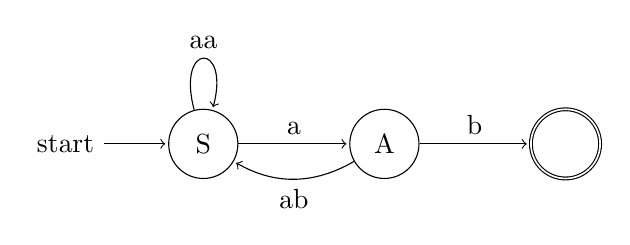
\begin{tikzpicture}[shorten >=1pt, scale=1.8, node distance=2.3cm, on grid, auto][t]
    \node[state, initial] (s) {S};
    \node[state] (a) [right=of s] {A};
    \node[state, accepting] (f) [right of=a] {};

    \path[->]   
    (s) edge[loop above] node {aa} (s)
        (s) edge node {a} (a)
    (a) edge[bend left] node {ab} (s)
        (a) edge node {b} (f);
\end{tikzpicture}
\newline
\noindent Splitting the transitions, we obtain the full FA.\\
\begin{tikzpicture}[shorten >=1pt, scale=1.8, node distance=2.3cm, on grid, auto][t]
    \node[state, initial] (s) {S};
    \node[state] (a) [right=of s] {A};
    \node[state] (aa) [above=of a] {};
    \node[state] (ss) [below=of s] {};
    \node[state, accepting] (f) [right of=a] {};

    \path[->]   
    (s) edge[bend left] node {a} (ss)
        (s) edge node {a} (a)
    (ss) edge[bend left] node {a} (s)
    (a) edge node {a} (aa)
        (a) edge node {b} (f)
    (aa) edge node[left=0.3cm] {b} (s);
\end{tikzpicture}
\newline
This is the final finite automaton that accepts the language above.
}

\pagebreak

% Cau 4

\qs{Answer the following question}{
    Construct a right-linear grammar that accept the language: \newline
    \indent \hspace{1cm} L = \{ w: w has both an even numberr of 0's and an even number of 1's \}
}

\sol{\newline
Define states:
\begin{itemize}
    \item $S$: w has even number of both 0 and 1
    \item $X_{0}$: w has odd number of 0
    \item $X_{1}$: w has odd number of 1
    \item $X_{01}$: w has odd number of both 0 and 1 
\end{itemize}
We construct a finite automaton to represent this language.
\newline
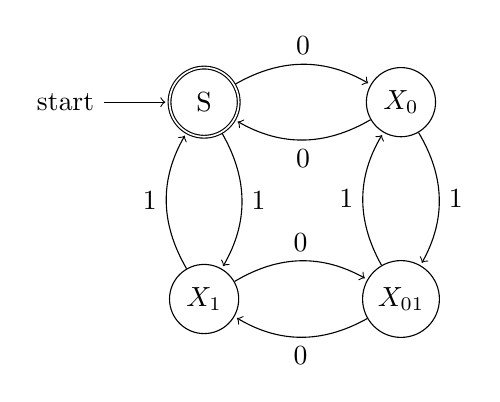
\begin{tikzpicture}[shorten >=1pt, scale=1.8, node distance=2.5cm, on grid, auto][t]
    \node[state, initial, accepting] (s) {S};
    \node[state] (x0) [right=of s] {$X_{0}$};
    \node[state] (x1) [below=of s] {$X_{1}$};
    \node[state] (x01) [below=of x0] {$X_{01}$};

    \path[->]   
    (s) edge[bend left] node {0} (x0)
        (s) edge[bend left] node {1} (x1)
    (x0) edge[bend left] node {0} (s)
        (x0) edge[bend left] node {1} (x01)
    (x1) edge[bend left] node {1} (s)
        (x1) edge[bend left] node {0} (x01)
    (x01) edge[bend left] node {0} (x1)
        (x01) edge[bend left] node {1} (x0);
\end{tikzpicture}
\newline
With this finite automaton, we can write a right-linear grammar:
\begin{equation*}
    \begin{aligned}
        &S &&\longrightarrow 0X_{0}~|~1X_{1}~|~\lambda \\
        &X_{0} &&\longrightarrow 0S~|~1X_{01} \\
        &X_{1} &&\longrightarrow 0X_{01}~|~1S \\
        &X_{01} &&\longrightarrow 0X_{1}~|~1X_{0}
    \end{aligned}
\end{equation*}
}
\end{document}
